% Scientific Data Data Descriptor. No journal template. No separate .bib/.bbl.
% Headings follow https://www.nature.com/sdata/submission-guidelines
% SNAPP Article (this instance): zip of this file plus figures/*.pdf only.
% Covering letter is a separate PDF and must not be in that zip.
% Author Contributions and Competing Interests are SNAPP form fields, not sections.
\documentclass[11pt,a4paper]{article}
\usepackage[T1]{fontenc}
\usepackage[utf8]{inputenc}
\usepackage{lmodern}
\usepackage{graphicx}
\usepackage{booktabs}
\usepackage{array}
\usepackage{tabularx}
\renewcommand{\tabularxcolumn}[1]{m{#1}}
\usepackage{amsmath}
\usepackage{microtype}
\usepackage[font=small,labelfont=bf,labelsep=period]{caption}
\captionsetup[figure]{name={Fig.}}
\captionsetup[table]{name={Table}}
\usepackage[margin=2.4cm,includefoot,footskip=16pt]{geometry}
\usepackage[section]{placeins}
\usepackage{setspace}
\usepackage{url}
\usepackage{xurl}
\usepackage[superscript,compress]{cite}
\usepackage[colorlinks=true,linkcolor=black,citecolor=black,urlcolor=blue,hypertexnames=false,bookmarks=false]{hyperref}
\urlstyle{same}
\onehalfspacing
\pagestyle{plain}
\pagenumbering{arabic}
\graphicspath{{figures/}{./}}
\newcommand{\thead}[1]{\multicolumn{1}{c}{#1}}

\title{A machine-checked proposition set for digital elevation model analysis}
\author{Yinggang Guo\\[0.4em]
\small Northwest Institute of Nuclear Technology, Xi'an 710024, China.\\
\small Correspondence: \mbox{\texttt{fariel\_gyg@163.com}}\\
\small ORCID: 0000-0002-8207-9941}
\date{}

\begin{document}
\maketitle

\begin{abstract}
This Data Descriptor deposits GeoProofBench v0.1, a \mbox{versioned} catalogue of
machine-checkable claims about digital elevation model (DEM) operators.
The release contains six concrete first-order propositions, five composition
or counter-example records, and forty-four stubbed identifiers reserved for
later entries. Each shipped claim has a stable identifier, a one-sentence
property, independent Dafny and Lean~4 specifications, a numerical gate, and
a recorded verdict. Operators include Wang--Liu pit filling and
deterministic eight-neighbour (D8) flow routing. Wolfram exhaustive checks and manim witnesses are
deposited where used; they are not required of every identifier. Custom code
is supplied only to regenerate those verdicts. The
deposit does not introduce a new interpolator. It records where a property
holds, where it fails as a property of the operator, and where resampling
is expected to break uniqueness. Input rasters include a $5\times5$ plane,
a $256\times256$ synthetic terrain, labelled synthetic stand-ins, and three
public product windows. Data are licensed CC-BY-4.0 and software MIT.
\end{abstract}

\section{Background \& Summary}

Three decades of DEM software have produced a shared analytical pipeline:
pit filling by the Wang--Liu spill rule (interior depressions are raised
to the lowest overflow)~\cite{wang2006}, flow direction, including
deterministic eight-neighbour (D8) routing~\cite{ocallaghan1984} and
flat-surface assignment~\cite{garbrecht1997}, watershed delineation, and
slope or curvature by Horn's $3\times3$ weighted fit or
Zevenbergen--Thorne profile curvature~\cite{horn1981,zevenbergen1987}. Each step is treated as correct
in an operational sense that is rarely written so that an independent
machine can check it. Independent GIS packages given the same raster can
return different flow fields and watershed maps~\cite{zhou2004}.
Algorithm choice still changes sink handling, extracted networks, and
river profiles~\cite{lindsay2016,schwanghart2017,clubb2017}. That
disagreement is not an academic curiosity: catchment area, stream length,
and outlet assignment feed flood mapping, infrastructure siting, and
published basin statistics. A single undeclared flat ring is enough to
invert a basin. GeoProofBench exists because those operators already
circulate as data products; what has been missing is a citable record of
the obligation each operator is supposed to meet.

The primary audience is the DEM and hydrology community that produces and
reuses those operators. Formal methods are the recording language, not the
subject of the deposit. Adjacent fields already treat numerical kernels as
proof obligations~\cite{boldo2009,melquiond2008,fumex2017,fulton2015,mitsch2017,zinzindohoue2017,leino2010,mathlib2020}.
DEM surfaces have also been used as input to linear temporal logic path
planners for ground vehicles~\cite{toscano2024}. That line of work
verifies a mission on a terrain, not the terrain operators themselves.
GeoProofBench is complementary: it archives the operator claims that a
later planner, model, or GIS tool may assume.

GeoAI and hydrology question-answering benchmarks
score agreement with an annotation or a textbook
answer~\cite{mai2024,kizilkaya2025}. Those resources remain useful for
language-level evaluation. GeoProofBench does not replace them. It supplies
the missing layer underneath: a proposition identifier that a model or a
GIS package can cite when it claims a geometric guarantee, rather than
when it matches a labelled answer. The same identifiers are named
obligations that a later automated reasoner, or a GeoMath-style agent
that cites DEM operators, can be scored against. This release does not
include a trained agent.

GeoProofBench is first a \emph{dataset}: a versioned set of proposition
records, rasters, metric tables, and verdicts. Data Records lists the
eleven shipped records (six first-order operators and five composition
or counter-example records) together with the deposit file layout.
Dafny, Lean~4, and Python files regenerate the required gates. Wolfram
exhaustive checks and manim witnesses are optional deposits, not part of
every record. None of that code is a substitute for the catalogue.
Identifiers GPB-006 to GPB-014 and
GPB-016 to GPB-050 are stubbed placeholders for community entries; they are not
implemented claims.
A related remote-sensing article~\cite{guo2025sam} does not share data
with this deposit.

\section{Methods}

\subsection{Proposition model}

Each shipped claim is checked on three independent tracks. Dafny and
Lean~4 state properties of the abstract operators (fill, D8, slope,
curvature) and prove lemmas about those specifications. The lemma counts
quoted later are proofs about those specs; they do not certify that a
particular Python file is the unique implementation. The reference
driver is a canonical Python re-implementation written against the spec.
Numerical gates check that this re-implementation, on the deposited
arrays, satisfies the spec's witness. The Python file is not the spec;
the spec is the Dafny and Lean file. The gates are finite tests, not
proofs. A record is labelled
PASS only when the numerical gates hold \emph{and} the corresponding
proof files verify. The two provers are independent restatements of the
same obligation; neither uses the Python driver as a test oracle for the
other. Wolfram exhaustive checks on small grids and manim witnesses are
deposited only where used.

Every shipped claim has a stable identifier, a one-sentence property, a
Dafny specification, an independent Lean~4 restatement, a Python
numerical gate, and a recorded verdict. The identifier, the property
sentence, the rasters, the metric JSON, and the verdict constitute the
data record. The proof and driver files are the regeneration procedure.

Further labels are not interchangeable with PASS:

\begin{itemize}
\item FP (failure of property): the claim is asserted on that input
  class, but the operator as specified does not satisfy it. The failure
  is unexpected relative to the hypothesis. It is not a software crash.
  This release records no FP instance. Version~0.1 ships obligations
  that hold on their stated class, plus documented counter-examples and
  one documented boundary (FAIL-TOLERANCE). An FP would be recorded if a
  claim that is asserted on a class then failed on an instance of that
  class.
\item FAIL-TOLERANCE: the input lies outside the claim's stated
  precondition, so the property is not asserted. It is not a licence for
  the operator to be wrong, and it is not an unexpected failure (that
  would be FP). In this release it is used only for the four
  $45^{\circ}$ cells of P-COMP-4. Unique D8 after resampling is claimed
  for a west-sloping plane at $0^{\circ}$ and $90^{\circ}$. At
  $45^{\circ}$, bilinear interpolation mixes cardinal neighbours, so
  unique D8 is not claimed. That $45^{\circ}$ mixing is a known GIS
  resampling boundary, not a GeoProofBench discovery. Those cells are excluded from the PASS tally
  and are not relabelled software FAIL.
\item NEGATIVE-RESULT PASS: a counter-example that is itself the
  intended record (unfilled four-ring; Zevenbergen--Thorne versus Horn).
\end{itemize}

\subsection{First-order operators}

Six operators are complete in this release (Table~\ref*{tab:operators}).
Pit filling follows the Wang--Liu spill rule~\cite{wang2006}: interior
pits are raised to the lowest overflow elevation. After that
fill, including its spill and index tie-breaking, D8 routing (O'Callaghan
and Mark's deterministic eight-neighbour rule) selects a
unique steepest downslope neighbour~\cite{ocallaghan1984} under a
strict-descent rule: a successor is recorded only when that neighbour is
strictly lower than the centre. If no strictly lower neighbour exists,
the cell is labelled NoFlow: it has no D8 successor. Watershed uniqueness is stated only after filling,
under that strict descent. The $5\times5$ teaching plane drops elevation
by $1$ at each flowing step because $A=1$ and $w=1$; P-COMP-1b has no
descent because the unfilled ring is flat.
Zevenbergen--Thorne profile curvature~\cite{zevenbergen1987} and Horn
second-order slope fitting~\cite{horn1981} are specified separately; they are
not treated as interchangeable (see Technical Validation).

\subsection{Composition}

P-COMP-1 states: after Wang--Liu filling, every interior cell under D8
has exactly one terminus. The argument uses five lemmas: filling yields
$\min(\mathrm{nbr})\le\mathrm{cell}$; D8 then descends; interior orbits
pigeonhole within $n\cdot m$ steps; a rectangular boundary supplies a
no-flow terminus; uniqueness collapses candidate termini. P-COMP-1b is
the complementary witness: an unfilled four-cell flat ring does not
terminate. P-COMP-2 instantiates the same chain on a $256^{2}$ constant
plane and on row slopes $\varepsilon\in\{10^{-6},10^{-4}\}$. P-COMP-4
resamples a west-sloping plane at scales $\{0.5,1,2,4\}\times$ and
rotations $\{0^{\circ},45^{\circ},90^{\circ}\}$. Its precondition is
rotation $\in\{0^{\circ},90^{\circ}\}$; unique D8 after resampling is
claimed only on those angles. The four $45^{\circ}$ cells lie outside that
precondition: bilinear interpolation mixes cardinal neighbours. That
mixing is a known GIS resampling boundary, not a GeoProofBench discovery.
P-COMP-5 checks
idempotence of filling and hash agreement of one-dimensional fill
outputs across Python, Dafny, and Lean. Idempotence
$\mathrm{fill}(\mathrm{fill}(h))=\mathrm{fill}(h)$ is claimed for
NoData-free rectangular rasters with finite real numbers.

Fig.~\ref*{fig:fill} is the teaching stencil for this chain. Panel a is
the unfilled four-cell flat ring (P-COMP-1b): D8 circulates and does not
terminate. Panel b is the $5\times5$ teaching plane
$h(p,q)=Ap+Bq+C$ with $A=1$ (elevation drop per cell toward decreasing
column index), $B=0$, and $C=12$ (centre elevation); $(p,q)$ are integer
offsets from the grid centre and the cell width is $w=1$. After filling,
flow is uniquely west-bound. Panel c diagrams the five-lemma order
recorded by the Dafny and Lean files; it is a map of the proof, not an
extra numerical gate. The multi-resolution stacks and the public windows
are Fig.~\ref*{fig:multi} and Fig.~\ref*{fig:real}; they are not this
stencil.

\begin{figure}[!htbp]
\centering
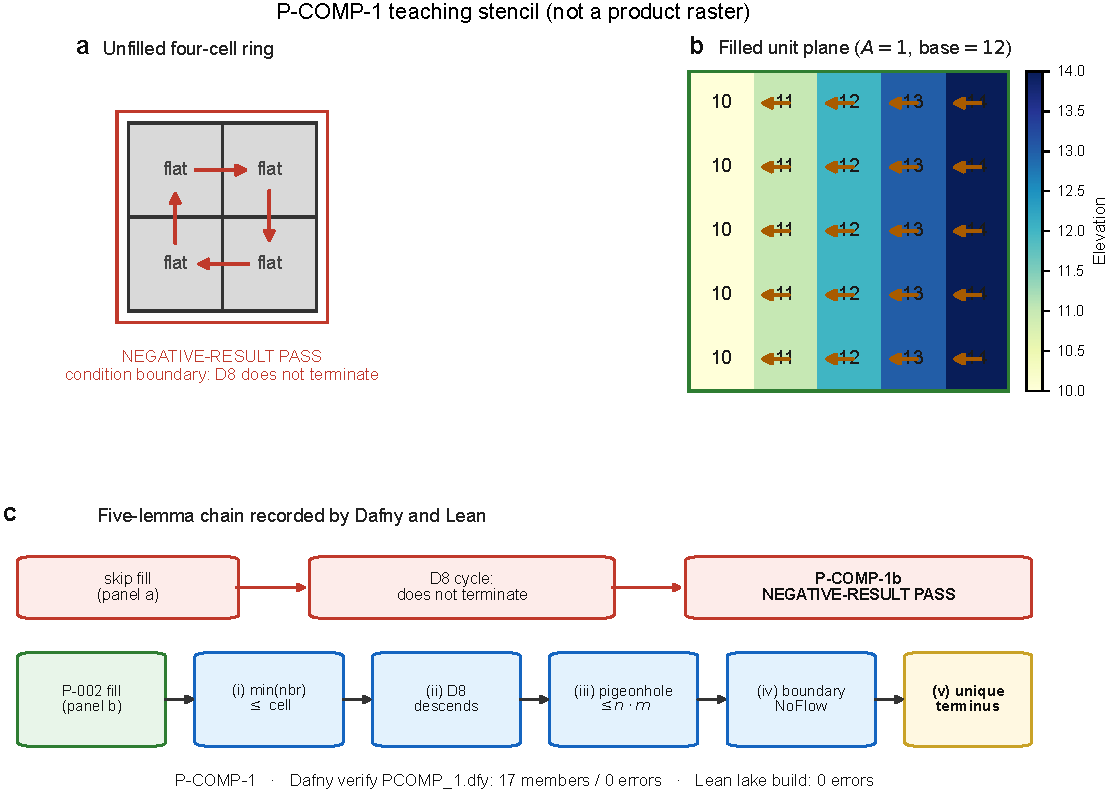
\includegraphics[width=\textwidth]{fig1_fill_watershed.pdf}
\caption{Teaching stencil for P-COMP-1.
(\textbf{a}) Condition-boundary counter-example (P-COMP-1b): unfilled
four-cell flat ring; D8 circulates and does not terminate.
(\textbf{b}) Filled $5\times5$ teaching plane
$h=Ap+Bq+C$ with $A=1$, $B=0$, $C=12$. Gold arrows mark unique
west-bound D8 successors.
(\textbf{c}) Five-lemma chain recorded by Dafny and Lean.
A cloud \texttt{dafny verify} of \texttt{PCOMP\_1.dfy} reports 17 verified
members / 0 errors for that compilation (file plus includes); Lean
\texttt{lake build} reports 0 errors. Panel~\textbf{a} and P-COMP-3 are
NEGATIVE-RESULT PASS records of different kinds.}
\label{fig:fill}
\end{figure}

\subsection{Input rasters}

Four stacks used in the multi-resolution harness are documented in
Table~\ref*{tab:dems}. Generation parameters for the three synthetic
arrays are in Table~\ref*{tab:synth}; the driver is
\texttt{p\_comp\_1\_multires.py} under \texttt{experiments/phase2/}.
That harness needs four grid sizes, including a $3601^{2}$ SRTM-shaped
array and a 4~m coarsened $256^{2}$ array. Intact public files at those
two sizes were not obtained from the author workstation. That is a
retrieval limit of this release, not a defect of SRTM or 3DEP. Copernicus
GLO-30 on tile N32E110 and the 3DEP ImageServer windows
(Table~\ref*{tab:real}, Fig.~\ref*{fig:real}) were obtained and are the
public-product checks. They do not replace the $3601^{2}$ size-stress
raster: a $256^{2}$ GLO-30 window is not a $3601^{2}$ SRTM tile. Version
0.1 therefore deposits labelled synthetic stand-ins for those two sizes.
A later version may add a true $3601^{2}$ SRTM tile; until then the
stand-ins are not a product-accuracy claim. The 1~m and 5~m windows were
taken from the 3DEP ImageServer nearest-neighbour export of those product
families, not from staged COG files (endpoints in Data Availability).
The three public products are a USGS 3DEP 1~m lidar-derived window
(Griffith Park, Los Angeles)~\cite{usgs3dep1m}, a USGS 3DEP 5~m Alaska
IFSAR window (Fairbanks area)~\cite{usgsifsar}, and a Copernicus DEM
GLO-30 window on tile N32E110~\cite{copernicusdem}.

Noise, when injected in other gates, uses
$\sigma\in\{0,10^{-3},10^{-2},10^{-1},0.5\}$~m.

\begin{table}[!htbp]
\centering
\caption{Synthetic raster generators (not product accuracy). All three
stand-ins are rebuilt by \texttt{p\_comp\_1\_multires.py}. Gaussian
$\sigma$ is in metres of elevation.}
\label{tab:synth}
\small
\begin{tabularx}{\textwidth}{>{\centering\arraybackslash}m{2.6cm}X}
\toprule
\thead{Stack} & \thead{Generator} \\
\midrule
terrain-A ($256^{2}$, 5~m) &
Ramp $0.05x+0.02y$, two Gaussian hills, twelve carved pits, then
$\mathcal{N}(0,5\times10^{-3})$ with NumPy integer seed
\texttt{20260906}
(\texttt{numpy.random.default\_rng}). \\
SRTM-scale ($3601^{2}$, 30~m) &
Used after the N32E110 \texttt{.hgt.gz} tile could not be retrieved intact.
$1180+0.035(3600-x)+85\sin(x/180)+55\cos(y/220)+25\sin((x+y)/95)$
plus $\mathcal{N}(0,1.6)$ with integer seed \texttt{11032}. \\
lidar-down ($256^{2}$, 4~m) &
Fine $1024^{2}$ field $0.04x+0.015y+4\sin(x/18)\cos(y/22)$
$+1.2\sin(x/3.5)+0.8\cos(y/4.2)$ plus $\mathcal{N}(0,0.25)$ with
integer seed \texttt{20260907}, then $4\times4$ block mean to $256^{2}$. \\
\bottomrule
\end{tabularx}
\end{table}

\subsection{Verification environment}

Numerical gates run on Python 3.12 (NumPy) on the author workstation.
Dafny 4.11 and Lean~4.18.0 with mathlib are re-executed from the
deposited sources on an independent AutoDL cloud mirror that does not
share the workstation's verifier cache; the lemma counts quoted below
are those cloud logs, not copies of local output. Wolfram Script 14 is
used only on the workstation (the cloud mirror has no Wolfram licence;
that skip is recorded, not treated as FAIL). Commands and file paths
live in the deposit under \texttt{experiments/} and \texttt{formal/}.

\subsection{Ethics}

No human participants, animals, or personal data were involved. Input
rasters are synthetic arrays or publicly distributed elevation products.

\section{Data Records}

While the formal specifications provide the highest recorded assurance,
the core data product---proposition statements, input rasters, metric
tables, and verdicts---can be used and cited independently of Dafny or
Lean. The citable object is the proposition catalogue
\texttt{GeoProofBench-v0.1\allowbreak-deposit.zip} at Science Data
Bank~\cite{gpbdata}. Table~\ref*{tab:catalog} lists the eleven shipped
records. Forty-four stubbed identifiers (GPB-006 to 014 and GPB-016 to
050) are reserved names in \texttt{benchmark/}; they are planned
extensions, not implemented claims in v0.1, and they are not rows of
that table. Table~\ref*{tab:files} is the deposit file layout. Data
Records describes the JSON, rasters, and metric tables; Code
Availability lists the Dafny, Lean, and Python regeneration files.

Metrics JSON live under
\texttt{experiments/phase2/results/} as \texttt{gpb021} (P-COMP-1),
\texttt{gpb024*} (multi-resolution), \texttt{gpb025*} (resampling),
\texttt{gpb026*} (hashes), and \texttt{gpb027\_realworld}.
Table~\ref*{tab:meta} is the field dictionary. In Table~\ref*{tab:dems}
the column $n_{\mathrm{out}}$ is the JSON field \texttt{uniq\_out}.
Table~\ref*{tab:real} lists the three public $256^{2}$ product windows.
Unless a suite states otherwise, \texttt{n\_term} and
\texttt{uniq\_out} are computed on the interior frame (excluding a
one-cell boundary).

\begin{table}[!htbp]
\centering
\caption{Dictionary for metrics JSON fields used in this Descriptor.}
\label{tab:meta}
\small
\begin{tabular}{ccm{1.6cm}m{6.8cm}}
\toprule
\thead{Field} & \thead{Type} & \thead{Unit} & \thead{Definition} \\
\midrule
\texttt{n\_pit} & integer & --- &
Count of interior 4-neighbour local minima on the unfilled raster. \\
\texttt{n\_term} & integer & --- &
Count of interior cells whose D8 orbit reaches a terminus. \\
\texttt{uniq\_out} & integer & --- &
Number of distinct termini among those terminating cells. \\
\texttt{longest} & integer & cell steps &
Length of the longest terminating D8 path. \\
\texttt{ridgeline\_frac} & float & 1 &
Fraction of interior cells with D8 in-degree 0. \\
\texttt{drainage\_density\_per\_m} & float & m$^{-1}$ &
Count of interior cells with in-degree $\ge 2$, divided by
(interior cell count $\times$ cell size). \\
\bottomrule
\end{tabular}
\end{table}

\begin{table}[!htbp]
\centering
\caption{Shipped GeoProofBench v0.1 records. Companions are noted, not
counted as extra first-order or composition identifiers.}
\label{tab:catalog}
\small
\begin{tabularx}{\textwidth}{cc>{\raggedright\arraybackslash}m{4.8cm}X}
\toprule
\thead{Status} & \thead{Count} & \thead{Identifiers} & \thead{Note} \\
\midrule
First-order & 6 & GPB-001 to 005 and GPB-015 &
GPB-002b is the 2-D companion of 002 (Table~\ref*{tab:operators});
it is not a seventh first-order identifier \\
Composition & 5 & P-COMP-1 to 5 &
P-COMP-1b is the unfilled-ring companion of 1 \\
\bottomrule
\end{tabularx}
\end{table}

\begin{table}[!htbp]
\centering
\caption{Deposit file layout (data products and regeneration sources).
SHA-256 hashes of the metrics JSON are in the named result files;
Lake caches are omitted.}
\label{tab:files}
\small
\begin{tabularx}{\textwidth}{>{\raggedright\arraybackslash}m{4.6cm}X}
\toprule
\thead{Path} & \thead{Contents} \\
\midrule
\texttt{experiments/}\newline\texttt{phase2/results/} &
Metrics JSON: \texttt{gpb021}, \texttt{gpb024*}, \texttt{gpb025*},
\texttt{gpb026*}, \texttt{gpb027\_realworld}. \\
\texttt{experiments/*/figures/} &
Optional mp4 witnesses where deposited. \\
\texttt{benchmark/} &
Identifier list, including forty-four planned-extension stubs. \\
\texttt{papers/P2-geoproofbench/} &
Descriptor text and figures. \\
\texttt{formal/dafny/*.dfy} &
13 Dafny specification files (Code Availability). \\
\texttt{formal/lean4/} &
VeriGIS library, \texttt{lakefile.toml}, \texttt{lean-toolchain}
(Code Availability). \\
\bottomrule
\end{tabularx}
\end{table}

\begin{table}[!htbp]
\centering
\caption{Shipped first-order operators and lead artefacts. GPB-002b is
the 2-D companion of GPB-002 and is not a seventh first-order
identifier. The six first-order records are GPB-001 to 005 and GPB-015.
GPB-015 uses the historical file prefix \texttt{P006} (watershed module);
the identifier is 015, not a mismatch with the six-record count.}
\label{tab:operators}
\begin{tabular}{cll}
\toprule
\thead{ID} & \thead{Property} & \thead{Lead Dafny file} \\
\midrule
GPB-001 & Slope sign on a plane & \texttt{P001\_horn\_slope.dfy} \\
GPB-002 & Pit filling to spill & \texttt{P002\_pit\_filling.dfy} \\
GPB-002b & 2-D fill monotone, idempotent & \texttt{P002\_pit\_filling\_2d.dfy} \\
GPB-003 & ZT curvature zero on a plane & \texttt{P003\_curvature.dfy} \\
GPB-004 & Horn fit exact on a plane & \texttt{P004\_consistency.dfy} \\
GPB-005 & Unique D8 successor & \texttt{P005\_d8.dfy} \\
GPB-015 & Watershed uniqueness under D8 & \texttt{P006\_watershed.dfy} \\
\bottomrule
\end{tabular}
\end{table}

\begin{table}[!htbp]
\centering
\caption{Multi-resolution stacks used with the same fill-then-D8 chain.
Asterisks mark synthetic stand-ins, not public elevation products.}
\label{tab:dems}
\begin{tabular}{crrrrr}
\toprule
\thead{Stack} & \thead{Grid} & \thead{$n_{\mathrm{pit}}$} &
\thead{$n_{\mathrm{term}}$} & \thead{$n_{\mathrm{out}}$} &
\thead{longest} \\
\midrule
plane-5~m & $5\times5$ & 0 & 9 & 3 & 3 \\
terrain-A & $256^{2}$ & 53 & 64516 & 98 & 351 \\
SRTM-scale stand-in$^{*}$ & $3601^{2}$ & 2519307 & 12952801 & 6027216 & 28 \\
lidar-down stand-in$^{*}$ & $256^{2}$ & 1782 & 64516 & 20137 & 13 \\
\bottomrule
\end{tabular}
\end{table}

\begin{table}[!htbp]
\centering
\caption{Public product windows deposited at $256^{2}$. Columns match the
metric JSON; P-COMP-1 gates all PASS. Ridge: interior D8 in-degree 0.
$D_d$: drainage density (m$^{-1}$).}
\label{tab:real}
\begin{tabular}{ccrrrr}
\toprule
\thead{Window} & \thead{Cell size} & \thead{$n_{\mathrm{pit}}$} &
\thead{$n_{\mathrm{out}}$} & \thead{ridge} & \thead{$D_d$} \\
\midrule
USGS 3DEP lidar, Griffith Park & 1~m & 88 & 234 & 0.125 & 0.106 \\
Alaska IFSAR, Fairbanks window & 5~m & 270 & 253 & 0.225 & 0.0363 \\
Copernicus GLO-30, N32E110 & 28.4~m & 626 & 4981 & 0.318 & 0.00685 \\
\bottomrule
\end{tabular}
\end{table}

\section{Data Overview}

Table~\ref*{tab:dems} and Fig.~\ref*{fig:multi} report fill-then-D8 on
four grid sizes. After filling, every interior cell terminates
($n_{\mathrm{term}}$ equals the interior count). Outlet count grows with
roughness and grid size (3 on the $5\times5$ plane; 98 on terrain-A;
$6.03\times10^{6}$ on the noisy SRTM-scale stand-in), while longest paths
do not (351 on terrain-A versus 13 on the lidar-down stand-in after
$4\times4$ block mean). Table~\ref*{tab:real} and Fig.~\ref*{fig:real}
apply the same gates to three public $256^{2}$ product windows; all three
PASS P-COMP-1 (zero interior pits after fill; 64\,516 / 64\,516 interior
cells terminate). Ridge fraction rises and drainage density falls as cell
size increases from 1~m lidar to 28.4~m GLO-30; that pattern is a
characteristic of these windows, not a general landscape claim.
Hydrologic users who need a named obligation for unique outlets after
filling can start from P-COMP-1; developers who need a named boundary for
rotated resampling should use the FAIL-TOLERANCE cells in Usage Notes.
Further summary statistics should be computed from the deposited arrays.

\begin{figure}[!htbp]
\centering
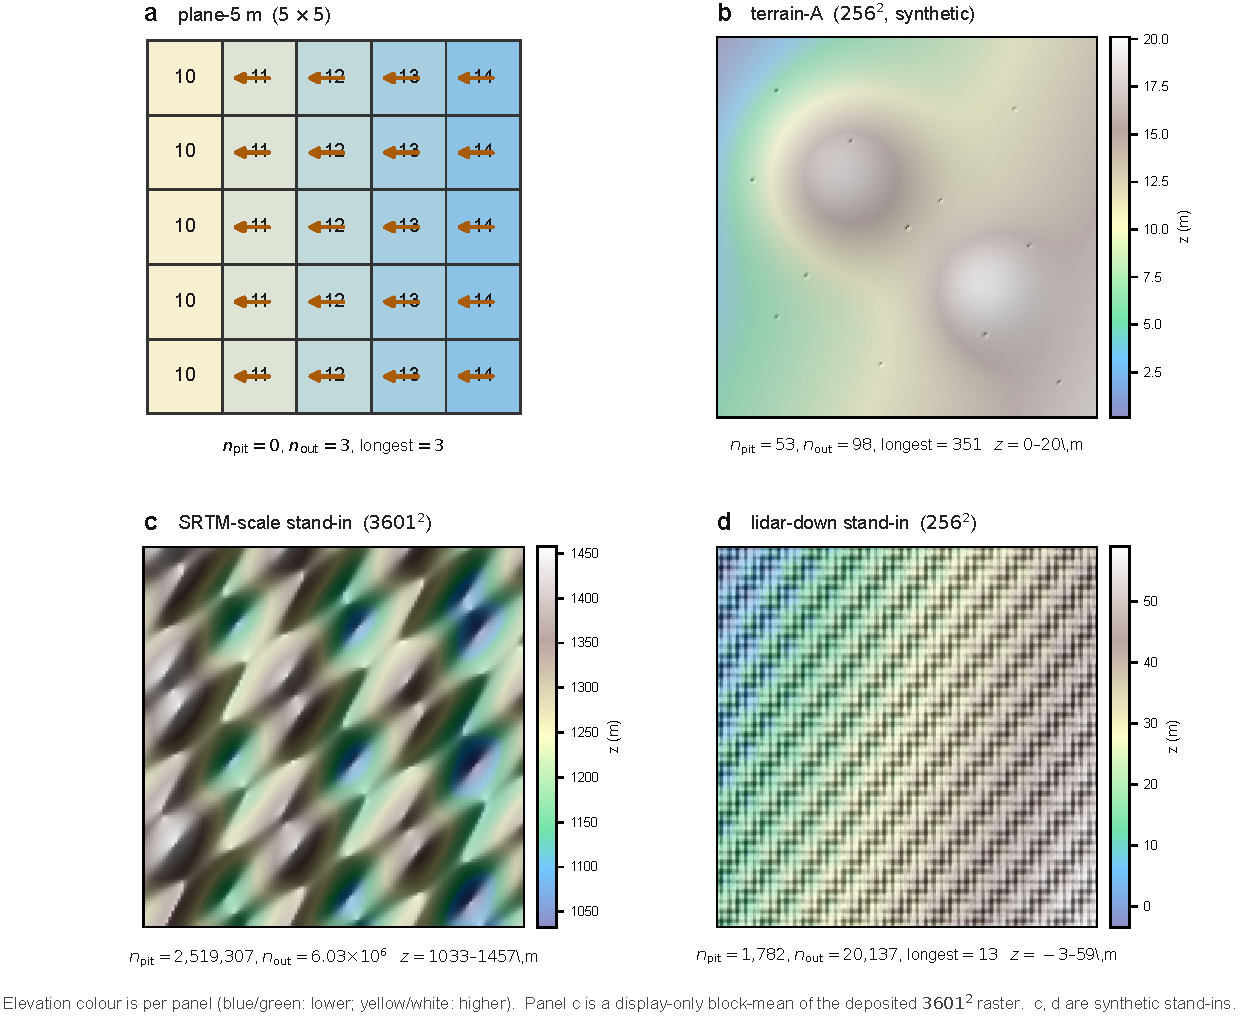
\includegraphics[width=\textwidth]{fig2_multires.pdf}
\caption{Fill-then-D8 inventory on the four deposited stacks.
(\textbf{a}) Unit plane, $5\times5$, shown as a labelled grid with D8
arrows (hillshade is undefined on a plane); cell numbers are elevation.
(\textbf{b}) Synthetic terrain-A, $256^{2}$.
(\textbf{c}) SRTM-scale stand-in. The deposited file is the full
$3601^{2}$ array; the panel is a display-only block-mean downsample,
not a substitute for that raster.
(\textbf{d}) Lidar-down stand-in, $256^{2}$; residual $4\times4$ block
structure after block mean at 4~m is a property of the deposited stack,
not a display artefact.
In \textbf{b}--\textbf{d}, colour maps elevation independently in each
panel (blue/green: lower; yellow/white: higher). $n_{\mathrm{pit}}$,
$n_{\mathrm{out}}$ and longest path are the deposited metrics. Panels
\textbf{c} and \textbf{d} are not public elevation products. Public
product windows are Fig.~\ref*{fig:real}.}
\label{fig:multi}
\end{figure}

\begin{figure}[!htbp]
\centering
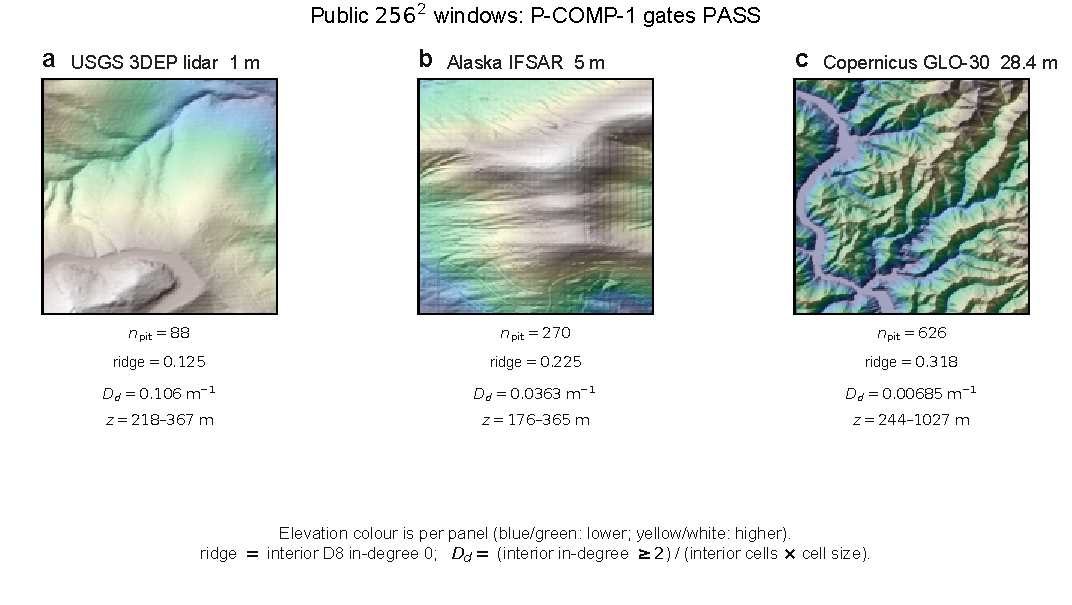
\includegraphics[width=\textwidth]{fig3_realworld.pdf}
\caption{Public $256^{2}$ windows used for diversity checks.
(\textbf{a}) USGS 3DEP 1~m lidar, Griffith Park.
(\textbf{b}) USGS 3DEP 5~m IFSAR, Fairbanks area.
(\textbf{c}) Copernicus GLO-30, tile N32E110.
Colour maps elevation independently in each panel (blue/green: lower;
yellow/white: higher) and is not a between-product height comparison.
Each panel reports interior pit count $n_{\mathrm{pit}}$, ridgeline
fraction (interior cells with D8 in-degree 0) and drainage density
$D_d$ (interior cells with in-degree $\ge 2$, divided by interior cell
count times cell size). All three windows PASS P-COMP-1.}
\label{fig:real}
\end{figure}

\section{Technical Validation}

Validation supports the technical quality of the deposited records. It is
not an analysis of a new terrain algorithm. Table~\ref*{tab:verdicts}
collects the gates that a user can regenerate from the archive.

\begin{table}[!htbp]
\centering
\caption{Summary of recorded verdicts. FAIL-TOLERANCE cells are excluded
from the PASS tally. This release records no FP instance.}
\label{tab:verdicts}
\begin{tabular}{cc}
\toprule
\thead{Record} & \thead{Verdict} \\
\midrule
P-COMP-1, $5\times5$ plane & PASS \\
P-COMP-1b four-ring & NEGATIVE-RESULT PASS \\
P-COMP-2 & PASS \\
P-COMP-3 & NEGATIVE-RESULT PASS \\
P-COMP-4 & 8 PASS + 4 FAIL-TOLERANCE (all $45^{\circ}$ rotations) \\
P-COMP-5 hashes / 2-D fill & 12/12 and 4/4 PASS \\
Three public windows & PASS \\
FP (this release) & none recorded \\
\bottomrule
\end{tabular}
\end{table}

\subsection{Numerical and formal gates}

On the $5\times5$ unit plane used for P-COMP-1 (Fig.~\ref*{fig:fill}\textbf{b}),
the record reports: no interior pit after fill; each flowing D8 step
drops elevation by $1$; all 9 interior cells terminate in at most 3
steps with 3 distinct outlets. On the author workstation, Wolfram enumeration of $4^{4}$ maps gives
\texttt{pigeonholeAll=true}, \texttt{descentAllFix=true},
\texttt{ringHasFixedPoint=false}. The AutoDL cloud mirror has no Wolfram
licence and skips that script; Python, Dafny, and Lean gates do not
depend on it.

An independent AutoDL cloud re-run of \texttt{dafny verify} on the
deposited files (no workstation cache) reports 17 verified members / 0
errors on \texttt{PCOMP\_1.dfy} and 12 / 0 on the termination file
\texttt{P006\_terminate\_under\_strict.dfy}. The same mirror reports
25 / 0 (\texttt{PCOMP\_2.dfy}), 20 / 0
(\texttt{PCOMP\_4\_homotopy.dfy}), and 15 / 0
(\texttt{PCOMP\_5\_idempotent.dfy}). Those integers are
verifier-reported members for each compilation unit (the named file plus
its \texttt{include}s). They are not lemma counts of GeoProofBench as a
whole. \texttt{PCOMP\_1.dfy} itself states 11 lemmas: five correspond to
steps (i)--(v) of Fig.~\ref*{fig:fill}\textbf{c}
(\texttt{NoPitImpliesDescent}, \texttt{D8PreservesDescent},
\texttt{OrbitLengthBound}, \texttt{BoundaryNonEmpty},
\texttt{FillThenWatershed}); the others are 2-D or pigeonhole variants,
uniqueness wrappers, and an example. Lean \texttt{lake build} of the
deposited \texttt{VeriGIS} library
against the locked mathlib was likewise executed on that mirror and
completes with 0 errors: the library builds. The lockfile imports 2764
mathlib modules; that number is a toolchain size, not a count of
GeoProofBench lemmas, and is not used as evidence that the propositions
hold.

P-COMP-2: a $256^{2}$ constant plane has 65536 / 65536 terminating cells
(all NoFlow). Row slopes $\varepsilon=10^{-6}$ and $10^{-4}$ terminate
with longest path 255 and 256 outlets (all north). The P-COMP-2 metrics JSON reports \texttt{visited\_cells} $=16\,908\,288$.
That field is a path-length sum, not a unique-cell census, and it is not
a column of Table~\ref*{tab:dems}. For each start cell the driver adds the
D8 path length in steps plus one (the start itself), then sums over all
$256^{2}$ starts in each suite. The constant plane contributes
$65\,536$. Each row-slope suite contributes $8\,421\,376$
($256\times(255\times256/2)+65\,536$). The three-suite total is
$16\,908\,288$.

P-COMP-4: 8 of 12 scale--rotation cells PASS with unique D8 and
$\sigma=0$. All four $45^{\circ}$ cells are FAIL-TOLERANCE as defined
above (precondition rotation $\in\{0^{\circ},90^{\circ}\}$). P-COMP-5:
four one-dimensional fill instances (plane, pit, slope,
cascade) are hashed with SHA-256 in Python, Dafny, and Lean. Agreement
on all 4 instances $\times$ 3 implementations is recorded as 12 / 12.
Two-dimensional $\mathrm{fill}(\mathrm{fill}(h))=\mathrm{fill}(h)$ holds
at $\sigma=0$ on four NoData-free rectangular rasters with finite real
numbers (4 / 4). A reversed heap-tie schedule is included: Wang--Liu
priority flood keys the heap by fill elevation then $(r,c)$; reversing
the sign of the $(r,c)$ components yields a second schedule. The two
outputs agree within the recorded epsilon.

P-COMP-1 on the three public windows: interior pits after fill are 0;
64516 / 64516 interior cells terminate (Table~\ref*{tab:real}).

\subsection{Counter-examples retained as records}

An unfilled 4-ring is a non-terminating D8 orbit (P-COMP-1b;
Fig.~\ref*{fig:fill}\textbf{a}): a condition-boundary counter-example that
marks where P-COMP-1 does not apply. Two $9\times9$ patches
$z=Dx^{2}+Ax$ show that Zevenbergen--Thorne profile curvature
$H_{xx}=2D$ and Horn's second-order coefficient $D_x=A$ are not the same
function (P-COMP-3; Fig.~\ref*{fig:zt}). The pairs
$(A,D)=(0.21,0.00705)$ and $(0.07,0.03485)$ were chosen so that both
centre-cell values are nonzero and need not vanish together; they are
not random draws. The figure is an existence witness, not a population
claim. Both records are catalogued as NEGATIVE-RESULT PASS.

\begin{figure}[!htbp]
\centering
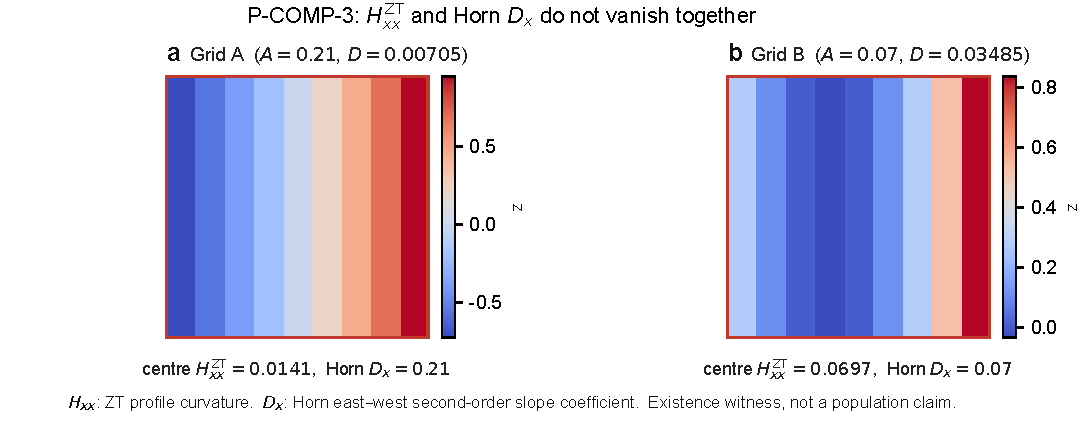
\includegraphics[width=\textwidth]{fig4_zt_horn.pdf}
\caption{Operator-inequivalence counter-example (P-COMP-3), a
NEGATIVE-RESULT PASS of a different kind from the condition-boundary
ring in Fig.~\ref*{fig:fill}\textbf{a}.
(\textbf{a}) Grid A: $z=Dx^{2}+Ax$ with $A=0.21$, $D=0.00705$.
(\textbf{b}) Grid B: $A=0.07$, $D=0.03485$.
$H_{xx}$ is Zevenbergen--Thorne profile curvature; $D_x$ is Horn's
east--west second-order slope coefficient. Centre-cell values are both
nonzero and do not vanish together, so the two operators are not
interchangeable. The grids demonstrate existence, not a population
claim.}
\label{fig:zt}
\end{figure}

\section{Usage Notes}

\subsection{Intended reuse}

Three entry points are intended.

DEM algorithm developers can attach a GPB identifier to a slope, fill,
D8, or watershed implementation and rerun the deposited Python gate on
their output raster. That path is sample testing: it checks finite
arrays, not a proof of the new code. A mismatch is a disagreement with a
named obligation, not with an unnamed laboratory convention.
The documented counter-examples (P-COMP-1b, P-COMP-3) are stress tests
for new algorithms: they mark edge cases that a conventional accuracy
score on a filled, well-sloped raster can miss.

Hydrologic modellers can cite P-COMP-1 when a workflow claims unique
outlets after filling, and can cite P-COMP-1b or the $45^{\circ}$
FAIL-TOLERANCE cells when a study area contains flats or rotated
resampling. The public-window metrics in Table~\ref*{tab:real} are
starting examples, not regional products.

Formal-methods researchers who need a machine-checked guarantee must
restate their operator against the deposited Dafny or Lean
specifications and rerun \texttt{dafny verify} or \texttt{lake build}.
The Lean restatement is independent of the Dafny kernel; agreement is a
cross-check, not a duplicated script. That embedding is the specialist
path; it is not required of GIS users who only rerun the Python gates.
Stubbed identifiers GPB-006 to GPB-014 and GPB-016 to GPB-050 are the
extension surface.

\subsection{How to run}

From the deposit root, each operator has a \texttt{run\_*.sh} (or the
matching \texttt{.py} on Windows). Formal files verify with
\texttt{dafny verify formal/dafny/<file>.dfy} and
\texttt{cd formal/lean4 \&\& lake build}. Lean~4.18.0 is pinned by
\texttt{formal/lean4/lean-toolchain}. Lake caches are not deposited;
the first \texttt{lake build} fetches mathlib from the lockfile (network
required; a cold cache takes on the order of tens of minutes).
Python drivers import NumPy and, for the public windows, GDAL; those
imports are the deposited dependency list. Wolfram scripts are optional.
Do not treat a missing Wolfram licence as a failed gate.

The $45^{\circ}$ resampling cells and the synthetic SRTM / lidar-down
rows are intentional boundaries. GPU parallel flow accumulation is not
in this release.

\section{Data Availability}

The Data Records section lists files and formats. The version of record
is openly available at Science Data Bank, V1~\cite{gpbdata}:
\url{https://doi.org/10.57760/sciencedb.011r9}
(CSTR \url{https://cstr.cn/31253.11.sciencedb.011r9};
identifier 31253.11.sciencedb.011r9).
Download is unrestricted. Data are licensed CC-BY-4.0 and software MIT.

Public rasters used as input were fetched as follows. USGS 3DEP windows
come from the ImageServer export
\url{https://elevation.nationalmap.gov/arcgis/rest/services/3DEPElevation/ImageServer/exportImage}
with \texttt{bboxSR=4326}, \texttt{imageSR=4326}, \texttt{size=256,256},
\texttt{format=tiff}, \texttt{interpolation=RSP\_NearestNeighbor}:
Griffith Park lidar (\texttt{west=-118.2964}, \texttt{south=34.1348},
cell 1~m)~\cite{usgs3dep1m} and Fairbanks IFSAR (\texttt{west=-147.815},
\texttt{south=64.894}, cell 5~m)~\cite{usgsifsar}. Copernicus GLO-30 tile
N32E110~\cite{copernicusdem} was read with GDAL \texttt{/vsicurl/} from
the public COG
\url{https://copernicus-dem-30m.s3.eu-central-1.amazonaws.com/Copernicus_DSM_COG_10_N32_00_E110_00_DEM/Copernicus_DSM_COG_10_N32_00_E110_00_DEM.tif}.

The work uses synthetic rasters and public elevation products only. It
does not involve human participants, personal data, or restricted
geographic holdings.

\section{Funding}

This research received no external funding and has no grant number. It
was supported by the author's institutional time at the Northwest
Institute of Nuclear Technology.

\section{Code Availability}

Custom code is included in the same archive as the data (MIT licence).
Dafny specifications live under \texttt{formal/dafny/} (13 files);
Lean~4 restatements under \texttt{formal/lean4/}
(\texttt{lakefile.toml}, \texttt{lean-toolchain}; Lake caches omitted);
Python and optional Wolfram drivers under \texttt{experiments/}.
Software versions used to generate the present verdicts: Python 3.12,
Dafny 4.11, Lean 4.18.0 with mathlib, NumPy, GDAL for windowed GeoTIFF
reads, manim 0.21 for animations. Public rasters are those listed under
Data Availability. The same tree is at
\url{https://github.com/fariell/verifiable-geocomputation}
(public development copy; Scientific Data is not double-blind).
Reviewers can download code from the unrestricted Science Data Bank zip
at the Data Availability DOI; a separate anonymised GitHub mirror is
not required.
No additional proprietary binaries are required for the numerical gates.

%% Author contributions and competing interests are captured on the SNAPP
%% web form and must not be duplicated as manuscript sections.

\begin{thebibliography}{30}
% Numbered in order of first citation in the text (Scientific Data).

\bibitem{wang2006}
Wang, L. \& Liu, H. An efficient method for identifying and filling surface depressions in digital elevation models for hydrologic analysis and modelling.
\textit{Int.\ J.\ Geogr.\ Inf.\ Sci.} \textbf{20}, 193--213 (2006).
\url{https://doi.org/10.1080/13658810500433453}

\bibitem{ocallaghan1984}
O'Callaghan, J. F. \& Mark, D. M. The extraction of drainage networks from digital elevation data.
\textit{Comput.\ Vis.\ Graph.\ Image Process.} \textbf{28}, 323--344 (1984).
\url{https://doi.org/10.1016/S0734-189X(84)80011-0}

\bibitem{garbrecht1997}
Garbrecht, J. \& Martz, L. W. The assignment of drainage direction over flat surfaces in raster digital elevation models.
\textit{J.\ Hydrol.} \textbf{193}, 204--213 (1997).
\url{https://doi.org/10.1016/S0022-1694(96)03138-1}

\bibitem{horn1981}
Horn, B. K. P. Hill shading and the reflectance map.
\textit{Proc.\ IEEE} \textbf{69}, 14--47 (1981).
\url{https://doi.org/10.1109/PROC.1981.11918}

\bibitem{zevenbergen1987}
Zevenbergen, L. W. \& Thorne, C. R. Quantitative analysis of land surface topography.
\textit{Earth Surf.\ Process.\ Landf.} \textbf{12}, 47--56 (1987).
\url{https://doi.org/10.1002/esp.3290120107}

\bibitem{zhou2004}
Zhou, Q. \& Liu, X. Error assessment of grid-based flow routing algorithms used in hydrological models.
\textit{Int.\ J.\ Geogr.\ Inf.\ Sci.} \textbf{18}, 319--338 (2004).
\url{https://doi.org/10.1080/13658810410001690444}

\bibitem{lindsay2016}
Lindsay, J. B. Efficient hybrid breaching-filling sink removal methods for flow path enforcement in digital elevation models.
\textit{Hydrol.\ Process.} \textbf{30}, 846--857 (2016).
\url{https://doi.org/10.1002/hyp.10648}

\bibitem{schwanghart2017}
Schwanghart, W. \& Scherler, D. Bumps in river profiles: uncertainty assessment and smoothing using quantile regression techniques.
\textit{Earth Surf.\ Dynam.} \textbf{5}, 821--839 (2017).
\url{https://doi.org/10.5194/esurf-5-821-2017}

\bibitem{clubb2017}
Clubb, F. J. \textit{et al.} Geomorphometric delineation of floodplains and terraces from objectively defined topographic thresholds.
\textit{Earth Surf.\ Dynam.} \textbf{5}, 369--385 (2017).
\url{https://doi.org/10.5194/esurf-5-369-2017}

\bibitem{boldo2009}
Boldo, S., Filli\^atre, J.-C. \& Melquiond, G. Combining Coq and Gappa for certifying floating-point programs in
\textit{Intelligent Computer Mathematics} (eds Carette, J., Dixon, L., Coen, C. S. \& Watt, S. M.)
59--73 (Springer, 2009).
\url{https://doi.org/10.1007/978-3-642-02614-0_10}

\bibitem{melquiond2008}
Melquiond, G. Proving bounds on real-valued functions with computations in
\textit{Automated Reasoning} (eds Armando, A., Baumgartner, P. \& Dowek, G.)
2--17 (Springer, 2008).
\url{https://doi.org/10.1007/978-3-540-71070-7_2}

\bibitem{fumex2017}
Fumex, C., March\'e, C. \& Moy, Y. Automating the verification of floating-point programs in
\textit{Verified Software: Theories, Tools, and Experiments}
(eds Paskevich, A. \& Wies, T.) 102--119 (Springer, 2018).
\url{https://doi.org/10.1007/978-3-319-72308-2_7}

\bibitem{fulton2015}
Fulton, N., Mitsch, S., Quesel, J.-D., V\"olp, M. \& Platzer, A.
KeYmaera~X: an axiomatic tactical theorem prover for hybrid systems in
\textit{Automated Deduction -- CADE-25}
(eds Felty, A. P. \& Middeldorp, A.) 527--538 (Springer, 2015).
\url{https://doi.org/10.1007/978-3-319-21401-6_36}

\bibitem{mitsch2017}
Mitsch, S. \& Platzer, A. ModelPlex: verified runtime validation of verified cyber-physical system models.
\textit{Form.\ Methods Syst.\ Des.} \textbf{49}, 33--74 (2016).
\url{https://doi.org/10.1007/s10703-016-0241-z}

\bibitem{zinzindohoue2017}
Zinzindohou\'e, J.-K., Bhargavan, K., Protzenko, J. \& Beurdouche, B.
HACL*: a verified modern cryptographic library in
\textit{Proc.\ 2017 ACM SIGSAC Conf.\ Computer and Communications Security}
1789--1806 (ACM, 2017).
\url{https://doi.org/10.1145/3133956.3134043}

\bibitem{leino2010}
Leino, K. R. M. Dafny: an automatic program verifier for functional correctness in
\textit{Logic for Programming, Artificial Intelligence, and Reasoning}
(eds Clarke, E. M. \& Voronkov, A.) 348--370 (Springer, 2010).
\url{https://doi.org/10.1007/978-3-642-17511-4_20}

\bibitem{mathlib2020}
The mathlib Community. The Lean mathematical library in
\textit{Proc.\ 9th ACM SIGPLAN Int.\ Conf.\ Certified Programs and Proofs}
367--381 (ACM, 2020).
\url{https://doi.org/10.1145/3372885.3373824}

\bibitem{toscano2024}
Toscano-Moreno, M., Mandow, A., Mart\'inez, M. A. \& Garc\'ia-Cerezo, A. J.
SPIN-based linear temporal logic path planning for ground vehicle missions with motion constraints on digital elevation models.
\textit{Sensors} \textbf{24}, 5166 (2024).
\url{https://doi.org/10.3390/s24165166}

\bibitem{mai2024}
Mai, G. \textit{et al.} On the opportunities and challenges of foundation models for GeoAI (vision paper).
\textit{ACM Trans.\ Spatial Algorithms Syst.} \textbf{10}, 11 (2024).
\url{https://doi.org/10.1145/3653070}

\bibitem{kizilkaya2025}
Kizilkaya, D., Sajja, R., Sermet, Y. \& Demir, I.
Toward HydroLLM: a benchmark dataset for hydrology-specific knowledge assessment for large language models.
\textit{Environ.\ Data Sci.} \textbf{4}, e31 (2025).
\url{https://doi.org/10.1017/eds.2025.10006}

\bibitem{guo2025sam}
Guo, Y., Liu, X., Rong, J., Shi, F. \& Tang, C.
SAM-GFNet: generalized feature fusion with hierarchical network for hyperspectral image semantic segmentation.
\textit{Remote Sens.} \textbf{17}, 3662 (2025).
\url{https://doi.org/10.3390/rs17223662}

\bibitem{usgs3dep1m}
National Geospatial Technical Operations Center, Earth Resources Observation and Science Center \& National Geospatial Program.
Seamless 1 meter Digital Elevation Models (DEMs) -- USGS National Map 3DEP Downloadable Data Collection.
U.S. Geological Survey \url{https://doi.org/10.5066/P13LJKFS} (2025).

\bibitem{usgsifsar}
U.S. Geological Survey, Earth Resources Observation and Science Center.
Digital elevation -- Interferometric synthetic aperture radar (IFSAR) -- Alaska.
U.S. Geological Survey \url{https://doi.org/10.5066/P9C064CO} (2013).

\bibitem{copernicusdem}
European Space Agency. Copernicus DEM -- Global and European Digital Elevation Model (COP-DEM).
\url{https://doi.org/10.5270/ESA-c5d3d65}

\bibitem{gpbdata}
Guo, Y. GeoProofBench v0.1: a machine-checked proposition set for digital elevation model analysis.
Science Data Bank \url{https://doi.org/10.57760/sciencedb.011r9} (2026).
CSTR: 31253.11.sciencedb.011r9.

\end{thebibliography}

\end{document}
